\documentclass[12pt]{beamer}
\usetheme{Penn} 
\usepackage{amsmath, amssymb, amsthm, amsfonts}
\usepackage{graphicx}
\usepackage{fancyvrb}
\usepackage{verbatim}
%\usepackage{tabularx}
\usepackage{tikz}
\usepackage{animate}
\usetikzlibrary{matrix, shapes, arrows, calc, backgrounds}
\usepackage[vcentermath, enableskew]{youngtab}
\newcommand{\ZZ}{\ensuremath{\mathbb{Z}}}
\newcommand{\RR}{\ensuremath{\mathbb{R}}}
\newcommand{\PP}{\ensuremath{\mathbb{P}}}

\newcommand{\CC}{\ensuremath{\mathbb{C}}}

\newtheorem{thm}{Theorem}[section]
\newtheorem{cor}[thm]{Corollary}
\newtheorem{lem}[thm]{Lemma}
\newtheorem{prop}[thm]{Proposition}
\theoremstyle{definition}
\newtheorem{conj}[thm]{Conjecture}
\newtheorem{defn}[thm]{Definition}
\newtheorem{ex}[thm]{Example}
\newtheorem{rmk}[thm]{Remark}
\newtheorem{alg}[thm]{Algorithm}
\newtheorem{question}[thm]{Question}
\begin{document}

\author[Z. Rosen]{Zvi Rosen \\ Department of Mathematics}

\date[\today]{\today}
\title[Optimization]{{\Large Single-Variable and Multivariate Optimization}}
\institute[Dept. of Mathematics~~--~~University of Pennsylvania]{}


\frame{\titlepage}

\begin{frame}
\frametitle{Task}
Given a function $f$ from $\RR \to \RR$, find the local
and global optima of the function.

\begin{defn}
Local Minimum (Maximum) is a point $x_0$ for which there exists $\epsilon > 0$
so that if $|x - x_0|<\epsilon$, then $f(x)\geq f(x_0)$ (resp. $f(x) \leq f(x_0)$).

Global Minimum (Maximum) is a point $x_0$ so that for any $x \in \RR$,
$f(x) \geq f(x_0)$ (resp. $f(x) \leq f(x_0)$.
\end{defn}
\end{frame}

\begin{frame}
\frametitle{Two techniques}
Two types of optimization techniques:
\begin{enumerate}
\item Gradient methods: Uses the derivative of 
the function.
\item Direct methods: Uses only function evaluation.
\end{enumerate}

\end{frame}

\begin{frame}
\frametitle{Single-variable gradient method}
Wherever the function $f$ has a local optimum $x_0$,
$f'(x_0) = 0$. \begin{itemize}
\item If $f''(x_0)>0$ then the function is convex or concave up. \\
The local optimum is a minimum.
\item If $f''(x_0)<0$, then the function is concave, or concave down. \\
The local optimum is a maximum.
\item If $f''(x_0) = 0$, then it may be a maximum, minimum or an inflection point. 
\end{itemize}
\end{frame}

\begin{frame}
\frametitle{Single-variable example}
Minimize $f(x) = e^x - x^3 - x$. \\

We compute $f'(x)= e^x - 3x^2 - 1$, and $f''(x) = e^x - 6x$. \\
One obvious root is $0$, which has $f''(0) > 0$ so it is a maximum. \\
Then we look for a root, using any root-finding method.
E.g. the{\tt fzero} method of MATLAB.

The root $3.7823$ has positive $f''(x)$ so it is a minimum. Further
argument shows that it is the global minimum.
\end{frame}

\begin{frame}
\frametitle{Gradient Descent}
Let $f(x,y)$ be a function of two variables. The gradient is:
\[\nabla f(x,y) = \left[ \begin{array}{c} f_x(x,y) \\ f_y(x,y) \end{array} \right]\]

The gradient is a vector pointing up, the negative gradient points down.

Iterate:
\[ x_{n+1} = x_n -\lambda_n \nabla f(x,y)\]
\end{frame}
\begin{frame}
\frametitle{Gradient Descent Example}
\[f(x,y) = 2x^2+2y^2-6x-6y+9\]
\[\nabla f(x,y) = \left[ \begin{array}{c} 4x -6 \\ 4y - 6 \end{array}\right]\]
Set $\lambda = .1$. Start at $(0,0)$.
\end{frame}

\begin{frame}
\frametitle{Direct Methods: Golden-Section Search}

Golden-section has a lot in common with the bisection method.

For optimization, computing the sign compared to the brackets is not enough.
We need to find the subinterval where the function is largest (resp. smallest).

So, at each step, we take two points inside the interval. Then, we take the
point with the larger value, and the two points on either side, and iterate.
\end{frame}

\begin{frame}
\frametitle{Direct Methods: Golden-Section Search}

{\bf Why is it called golden-section?}

We want to save time by only computing one new function value
at each iteration.

\vspace{5mm}

In particular, we want $\frac{\ell}{s} = \frac{s}{\ell-s}$, with
$\ell + s = 1$.
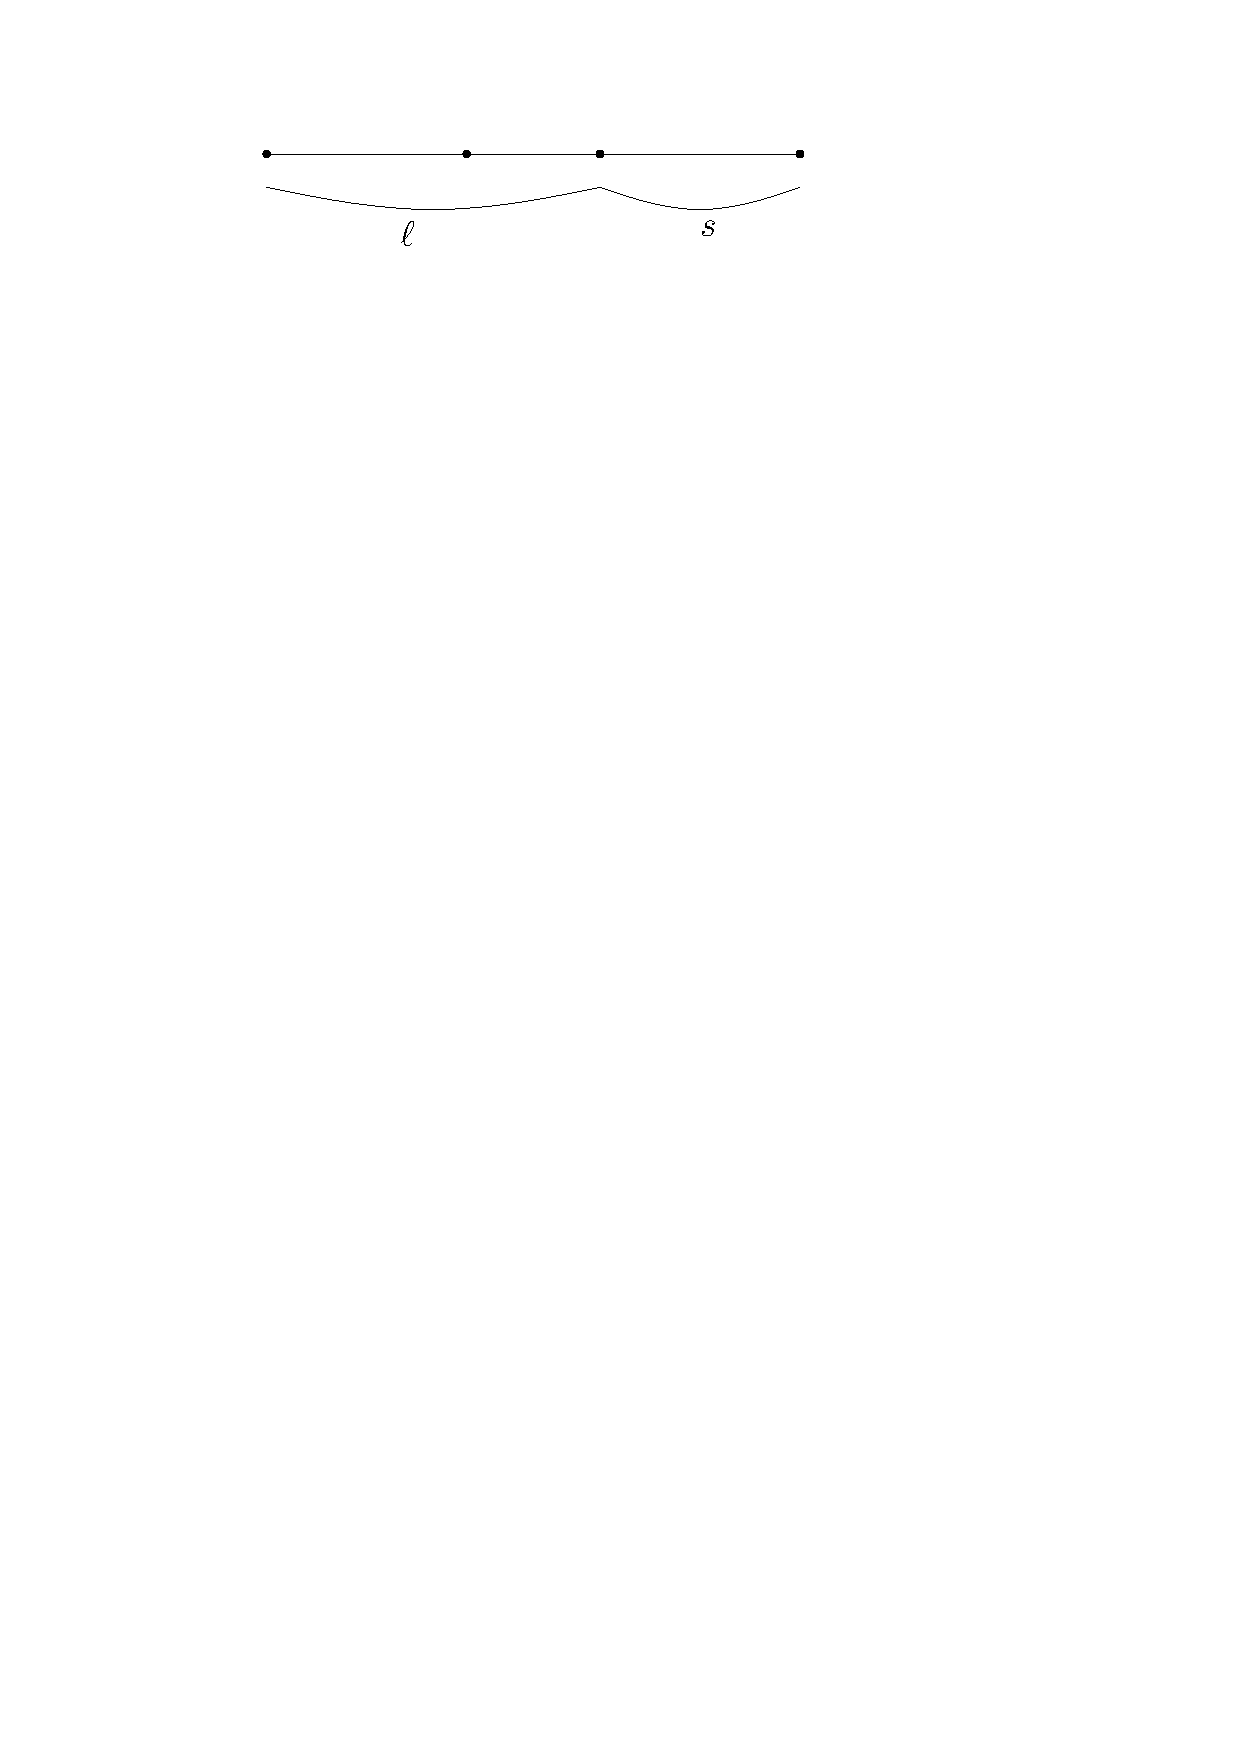
\includegraphics{opt-fig.pdf}



{\bf What if our bracket contains multiple local optima?} Golden
section will not work.
\end{frame}
\begin{frame}
\frametitle{Parabolic Interpolation}

Begin with three points $x_1x_2,x_3$, two of which bracket the true maximum (resp. minimum). Suppose $x_1$ is the left endpoint and $x_2$ is the right
endpoint.

There is a unique parabola that contains the three points. Find its maximum.
Then add that point as $x_4$. For the next iteration, use the three
consecutive points for which $f($midpoint$)$ is largest.
\end{frame}

\begin{frame}
\frametitle{Parabolic Interpolation}

Begin with three points $x_1x_2,x_3$, two of which bracket the true maximum (resp. minimum). Suppose $x_1$ is the left endpoint and $x_2$ is the right
endpoint.

There is a unique parabola that contains the three points. Find its maximum.
Then add that point as $x_4$. For the next iteration, use the three
consecutive points for which $f($midpoint$)$ is largest.
\end{frame}

\begin{frame}
\frametitle{Parabolic Interpolation - Example}
Maximize $f(x) = \sin(x)$. Let $x_1 = 0, x_2 = 1, x_3 = 2$. The corresponding
sine values are $0, 0.84, 0.91$.

The parabola has formula 
\[y = (x -0)(x-1)\frac{0.91}{2} + (x -0)(x-2)\frac{0.84}{-1}
+ (x-1)(x-2)\frac{0}{2}\]
\[ = 1.225 x-0.385 x^2.
\]
The maximum of this parabola is reached at 
$x_4 = 1.225/(2\cdot 0.385) = 1.59$.
The value of sine at this point is $0.9998$. In the next iteration, we 
would use $x_2,x_4$, and $x_3$.
\end{frame}
\begin{frame}
\frametitle{Nelder-Mead Algorithm}

Implemented in MATLAB using {\tt fminsearch}.

See gif.
\end{frame}



\end{document}
